\documentclass[11pt, a4]{article}
\usepackage{geometry}
\geometry{margin=1.25in}
\usepackage[utf8]{inputenc}
\usepackage[english]{babel}
\usepackage{amsmath}
\usepackage{graphicx}
\graphicspath{ {../figures/} }
\usepackage{placeins}

\title{Supermarket sales \\
		\large Exploratory Data Analysis for Machine Learning - Course Project}
\author{Caio Mescouto Terra de Souza}
\date{\today}

\begin{document}

\maketitle

\section*{Brief Description of the Data Set and a Summary of its Attributes}

Supermarket sales data set \cite{sales} is a historical record of sales data in 3 different Branches for 3 months. Each observation has 17 features that indicates where the purchase happen (Branch, City), when (Date and Time), the Product Line, Unit Price, Quantity, Payment method, Cost of goods sold, margins, Taxes and Customer informations (Gender and Type) in addition to stratification rating on their overall shopping experience.

The data set has 1000 observations and no missing values. The variables are presented below:

- Invoice id: Computer generated sales slip invoice identification number

- Branch: Branch of supercenter (3 branches are available identified by A, B and C).

- City: Location of supercenters

- Customer type: Type of customers, recorded by Members for customers using member card and Normal for without member card.

- Gender: Gender type of customer

- Product line: General item categorization groups - Electronic accessories, Fashion accessories, Food and beverages, Health and beauty, Home and lifestyle, Sports and travel

- Unit price: Price of each product in \$

- Quantity: Number of products purchased by customer

- Tax: 5\% tax fee for customer buying

- Total: Total price including tax

- Date: Date of purchase (Record available from January 2019 to March 2019)

- Time: Purchase time (10am to 9pm)

- Payment: Payment used by customer for purchase (3 methods are available – Cash, Credit card and Ewallet)

- COGS: Cost of goods sold

- Gross margin percentage: Gross margin percentage

- Gross income: Gross income

- Rating: Customer stratification rating on their overall shopping experience (On a scale of 1 to 10)


\section*{Initial Plan for Data Exploration}

At the very first glimpse on the data set it was identified that Branch and City have the same information, so we will keep only one for the analysis. Tax and gross margin have no variance, the exploratory data analysis on margins or taxes are not meaningful and we will drop all related variables. Additionally, Date and Time will be merged as a Timestamp that is easily manipulated. 

Considering this information, the plan has three main lines of investigation: customers and purchase, differences between branches and seasonalities (day of the week or time of the day).

- Customers are divided by gender and type (member or normal) and purchase has quantity, unit price and total, besides Product line. We will focus on Customer and Product line to seek some differences in Total.

- With seasonalities the focus will be on Total and Rating.

- For Branches the focous will be in differences in the Total.
 

\section*{Data Cleaning and Feature Engineering}


The data set does not have missing data or outliers that could indicate problematic attributes or observation. As stated before some attributes were dropped and Date and Time was merged as timestamps. The attribute “Total” that represents the total purchase value is right skewed (Figure \ref{fig:hist}), so the log transformation was applied. Other numerical variables are equally distributed, by now no feature engineering was applied, but could require some standardization for machine learning purposes.

\begin{figure}[!h]
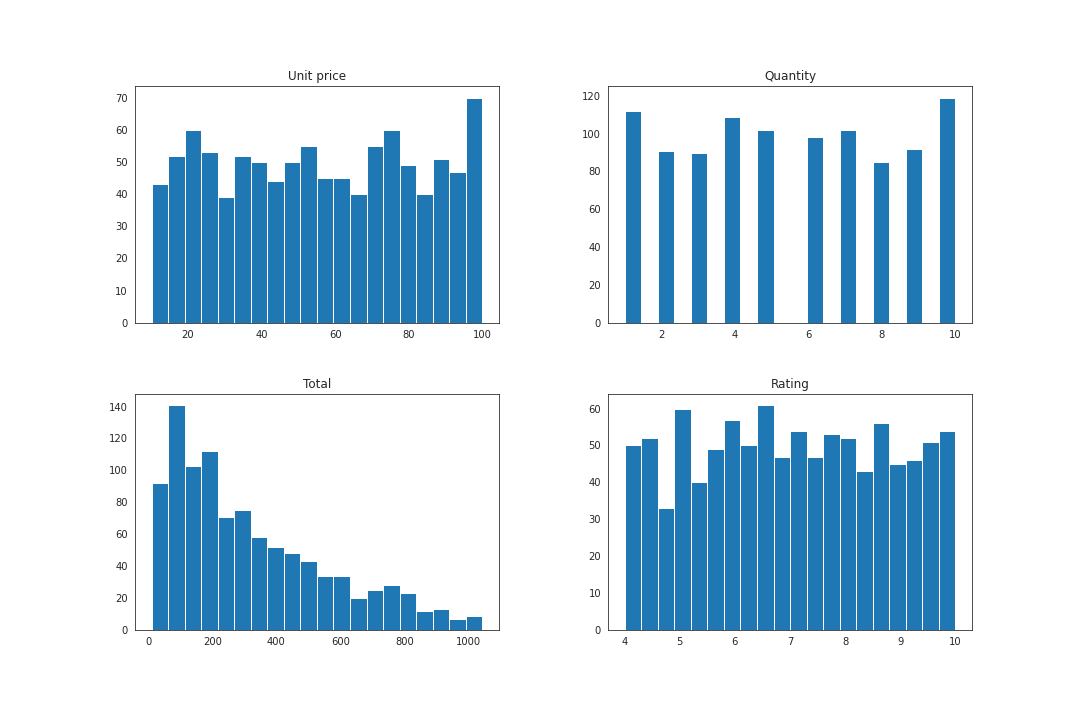
\includegraphics[scale=0.35]{hist}
\centering
\caption{Histograms}
\label{fig:hist}
\end{figure}


The categorical variables have small numbers of categories and are good candidates for one hot encoding as they are not ranked.

\section*{Key Findings and Insights}

Besides Quantity, Unit Price and Total, the numerical attributes do not have strong correlation between them. Also the distribution by categories were tested and any strong deviation was observed.

Meaningful insights are found looking into categorical attributes. For example, men spent more in Health and beauty than women in total amount and proportion (Figure \ref{fig:box}). The average spent in Cash is bigger than others payment methods except for Electronic accessories and Sports and travel.

\begin{figure}[!h]
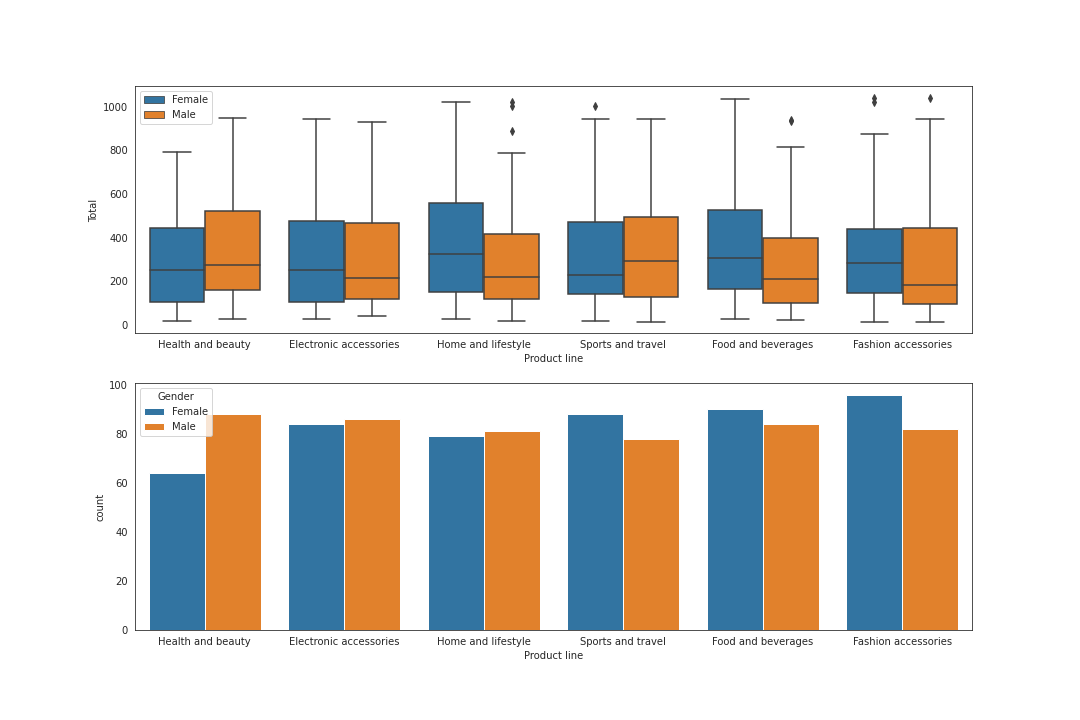
\includegraphics[scale=0.35]{boxgender}
\centering
\caption{Gender and Product line}
\label{fig:box}
\end{figure}

\begin{figure}[!h]
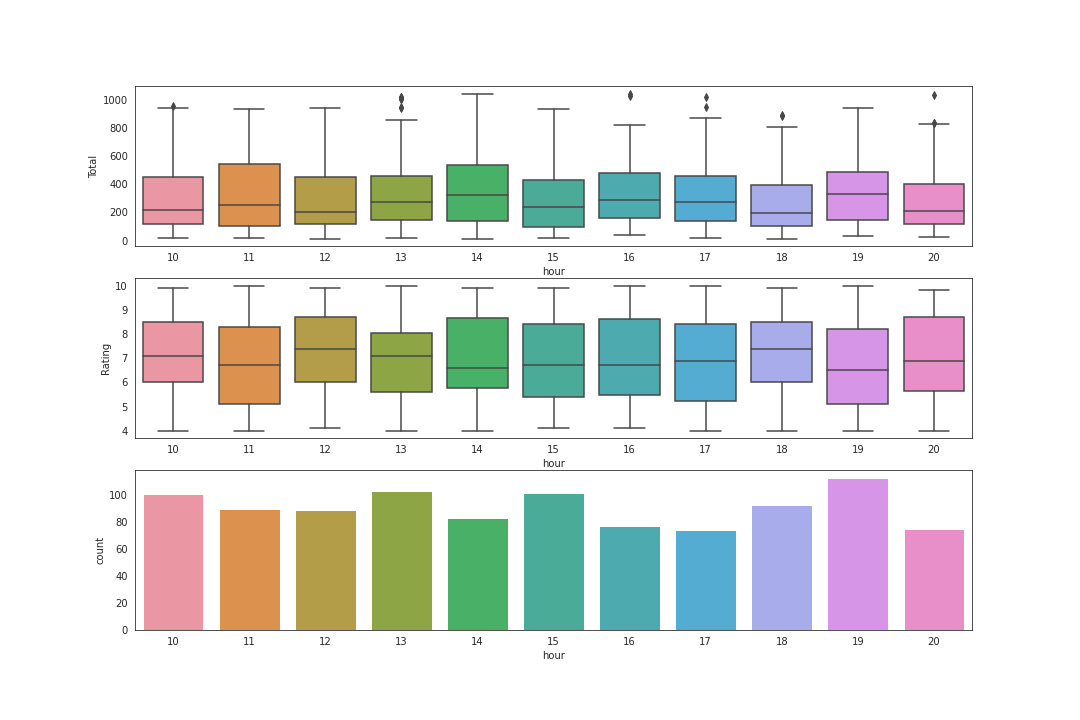
\includegraphics[scale=0.35]{hour}
\centering
\caption{Purchases per hour of the day}
\label{fig:hour}
\end{figure}

\begin{figure}
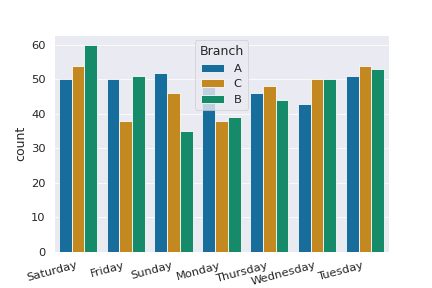
\includegraphics[scale=0.35]{week}
\centering
\caption{Rating per day of the week}
\label{fig:week}
\end{figure}


Moving on to seasonality issues, 19:00 is the hour with the greatest amount of purchases and with the second highest mean total value, but with the lowest mean evaluation (Figure \ref{fig:hour}) and Monday is the day of less purchases but highest rating (Figure \ref{fig:week}).



\section*{Main Hypotheses}

Considering the insights presented in the preceding section, we can formulate some hypotheses.

\begin{itemize}
\item The average men purchase in Health and beauty is bigger than women;\\
\item The average 19:00 rating is lower than the rest of the hours;\\
\item Monday's movement is less than in the rest of the week.

\end{itemize}

\section*{Significance Test}

To test one of those hypotheses, a formal significance test was carried out for the first hypothesis raised. As the distributions are not normal, but have similar shape (Figure \ref{fig:test}), the \textit{Mann-Whitney} non-parametric test was applied and the result is presented below. 

\begin{figure}
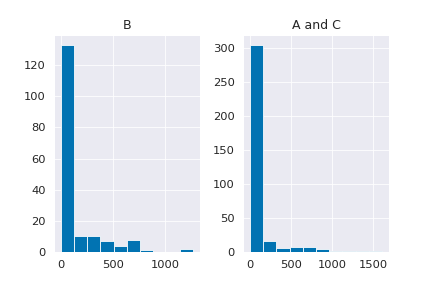
\includegraphics[scale=0.35]{test}
\centering
\caption{Total histogram}
\label{fig:test}
\end{figure}

\begin{align*}
&\alpha = 0.05\\
&H_0: \text{Gender has no effect on purchase value for Health and beauty products}  \\
&H_1:\text{Purchase value for Health and beauty products is different between Gender}\\
& p-value=0.1761 > \alpha\\
\end{align*}

As the $p-value$ is greater than $\alpha$, the null hypothesis cannot be rejected.

\section*{Next Steps}

Seasonalities can be a good topic to investigate more, the relationship with ratings on days of the week and hours can indicate some issues, for example few employees helping customers during rush hours, or a specific employee group that are not well trained in customer assistance. 

\section*{Coments About the Data Set}

The data set has a time constraint for example for forecasting demand, another problem is the level of information related to products, only the big lines are available and further investigations on consumptions are impossible. In addition, Customer ID can help with suggestion algorithms. Finally, the information about Tax and Cost are meaningless and any analysis on costs and earnings is impossible from this data set. 

\FloatBarrier

\begin{thebibliography}{9}

\bibitem{sales} 
Supermarket sales:
Historical record of sales data in 3 different supermarkets,
\\\texttt{https://www.kaggle.com/aungpyaeap/supermarket-sales}
\end{thebibliography}

\end{document}